%%--------------------!TeX program = xelatex--------------------%%
\documentclass[9pt]{book}

\usepackage{SJTUSFFABook}

%%--------------------正文开始--------------------%%
\begin{document}

%% 无页码
\frontmatter
%%--------------------扉页--------------------%%
\begin{titlepage}
  \centering
  \vspace*{7cm}
  {\Huge\bfseries \songti 生命在于瞎折腾} \\
  \vfill
  {\fzxztfw 上海交通大学科幻奇幻协会}
\end{titlepage}

%%--------------------空白页--------------------%%
\clearpage
\thispagestyle{empty} % 只影响当前页
\null
\newpage

%%--------------------目录--------------------%%
\begingroup
  \pagestyle{empty}
  \tableofcontents
  \thispagestyle{empty}
\endgroup

%%--------------------空白页--------------------%%
\clearpage
\thispagestyle{empty} % 只影响当前页
\null
\newpage

%% 页码开始
\mainmatter

%%--------------------卷首语--------------------%%
\newpage
\myheadertext{卷首语}{English Book Name|社刊中文名} % 自定义页眉
\phantomsection % 添加到目录
\addcontentsline{toc}{chapter}{卷首语}

\vspace*{-2em}
\noindent % 取消缩进
\parbox[t][1in][c]{\textwidth}{% 指定高度、对齐方式和宽度
    {\Huge \bfseries 卷首语标题}
    \par
    \normalsize
    \vspace{2em}
    {文 $\_$ 作者}
}
\vspace*{4em}

\section*{模板说明}
本模板为上海交通大学科幻奇幻协会社刊模板。

默认模板文件由以下部分组成:

\begin{itemize}
    \item \texttt{main.tex} 主文件
    \item \texttt{SJTUReport.sty} 版式控制,包括一些基础的设置,如版面、字体、页眉、标题等
    \item \texttt{figures} 放置图片的文件夹
    \item \texttt{fonts} 放置字体的文件夹
\end{itemize}

\section*{发布地址}
\begin{itemize}
    \item Github: \url{https://github.com/gpabooks/SJTUSFFA-Book-Template}
    \item Overleaf:  \url{https://www.overleaf.com/latex/}
\end{itemize}

\zhlipsum[1-2]

\vspace{1\baselineskip}
{\hfill 2002年5月22日}

% 示例图标
\vspace*{\fill}
\begin{center}
  \scalebox{8.0}{%
    \textcolor{black!30}{%
      \faIcon[regular]{hand-spock}%  
    }%
}
\end{center}
\vfill

%%--------------------版块起始页面--------------------%%
\newpage
\chapterstartpage{English Chapter Name}{在\\此\\的\\版\\块\\名}{在目录中显示的版块名}

%%--------------------内容--------------------%%
\newpage
\myheadertext{右页眉篇目名}{English Chapter Name |左页眉版块名}
\sectionwithsubtitle{在此显示的小说标题}{文 $\_$ 作者\quad 译 $\_$ 译者}{在目录中显示的小说标题}
\begin{multicols}{2}

\noindent

\subsection*{一\quad 章节名}
正文文本
\par
\zhlipsum[1]

\subsubsection*{一\quad 小节名}
\zhlipsum[2]

\begin{myquotation}
引用示例
\par
\zhlipsum[3]
\end{myquotation}

\zhlipsum[4]

脚注示例\footnote[1]{这是一个脚注}。

\zhlipsum[5-7]

\end{multicols}

\vspace*{\fill}
\begin{center}
\kaishu 生生不息,繁荣昌盛
\end{center}
\vfill


\newpage
\chapterstartpage{English Chapter Name}{漫\\画\\·\\笑\\话}{漫画·笑话}

\newpage
\myheadertext{漫画标题}{English Chapter Name |漫画·笑话}
\phantomsection
\addcontentsline{toc}{section}{漫画标题}
\begin{figure}[H]
  \centering
  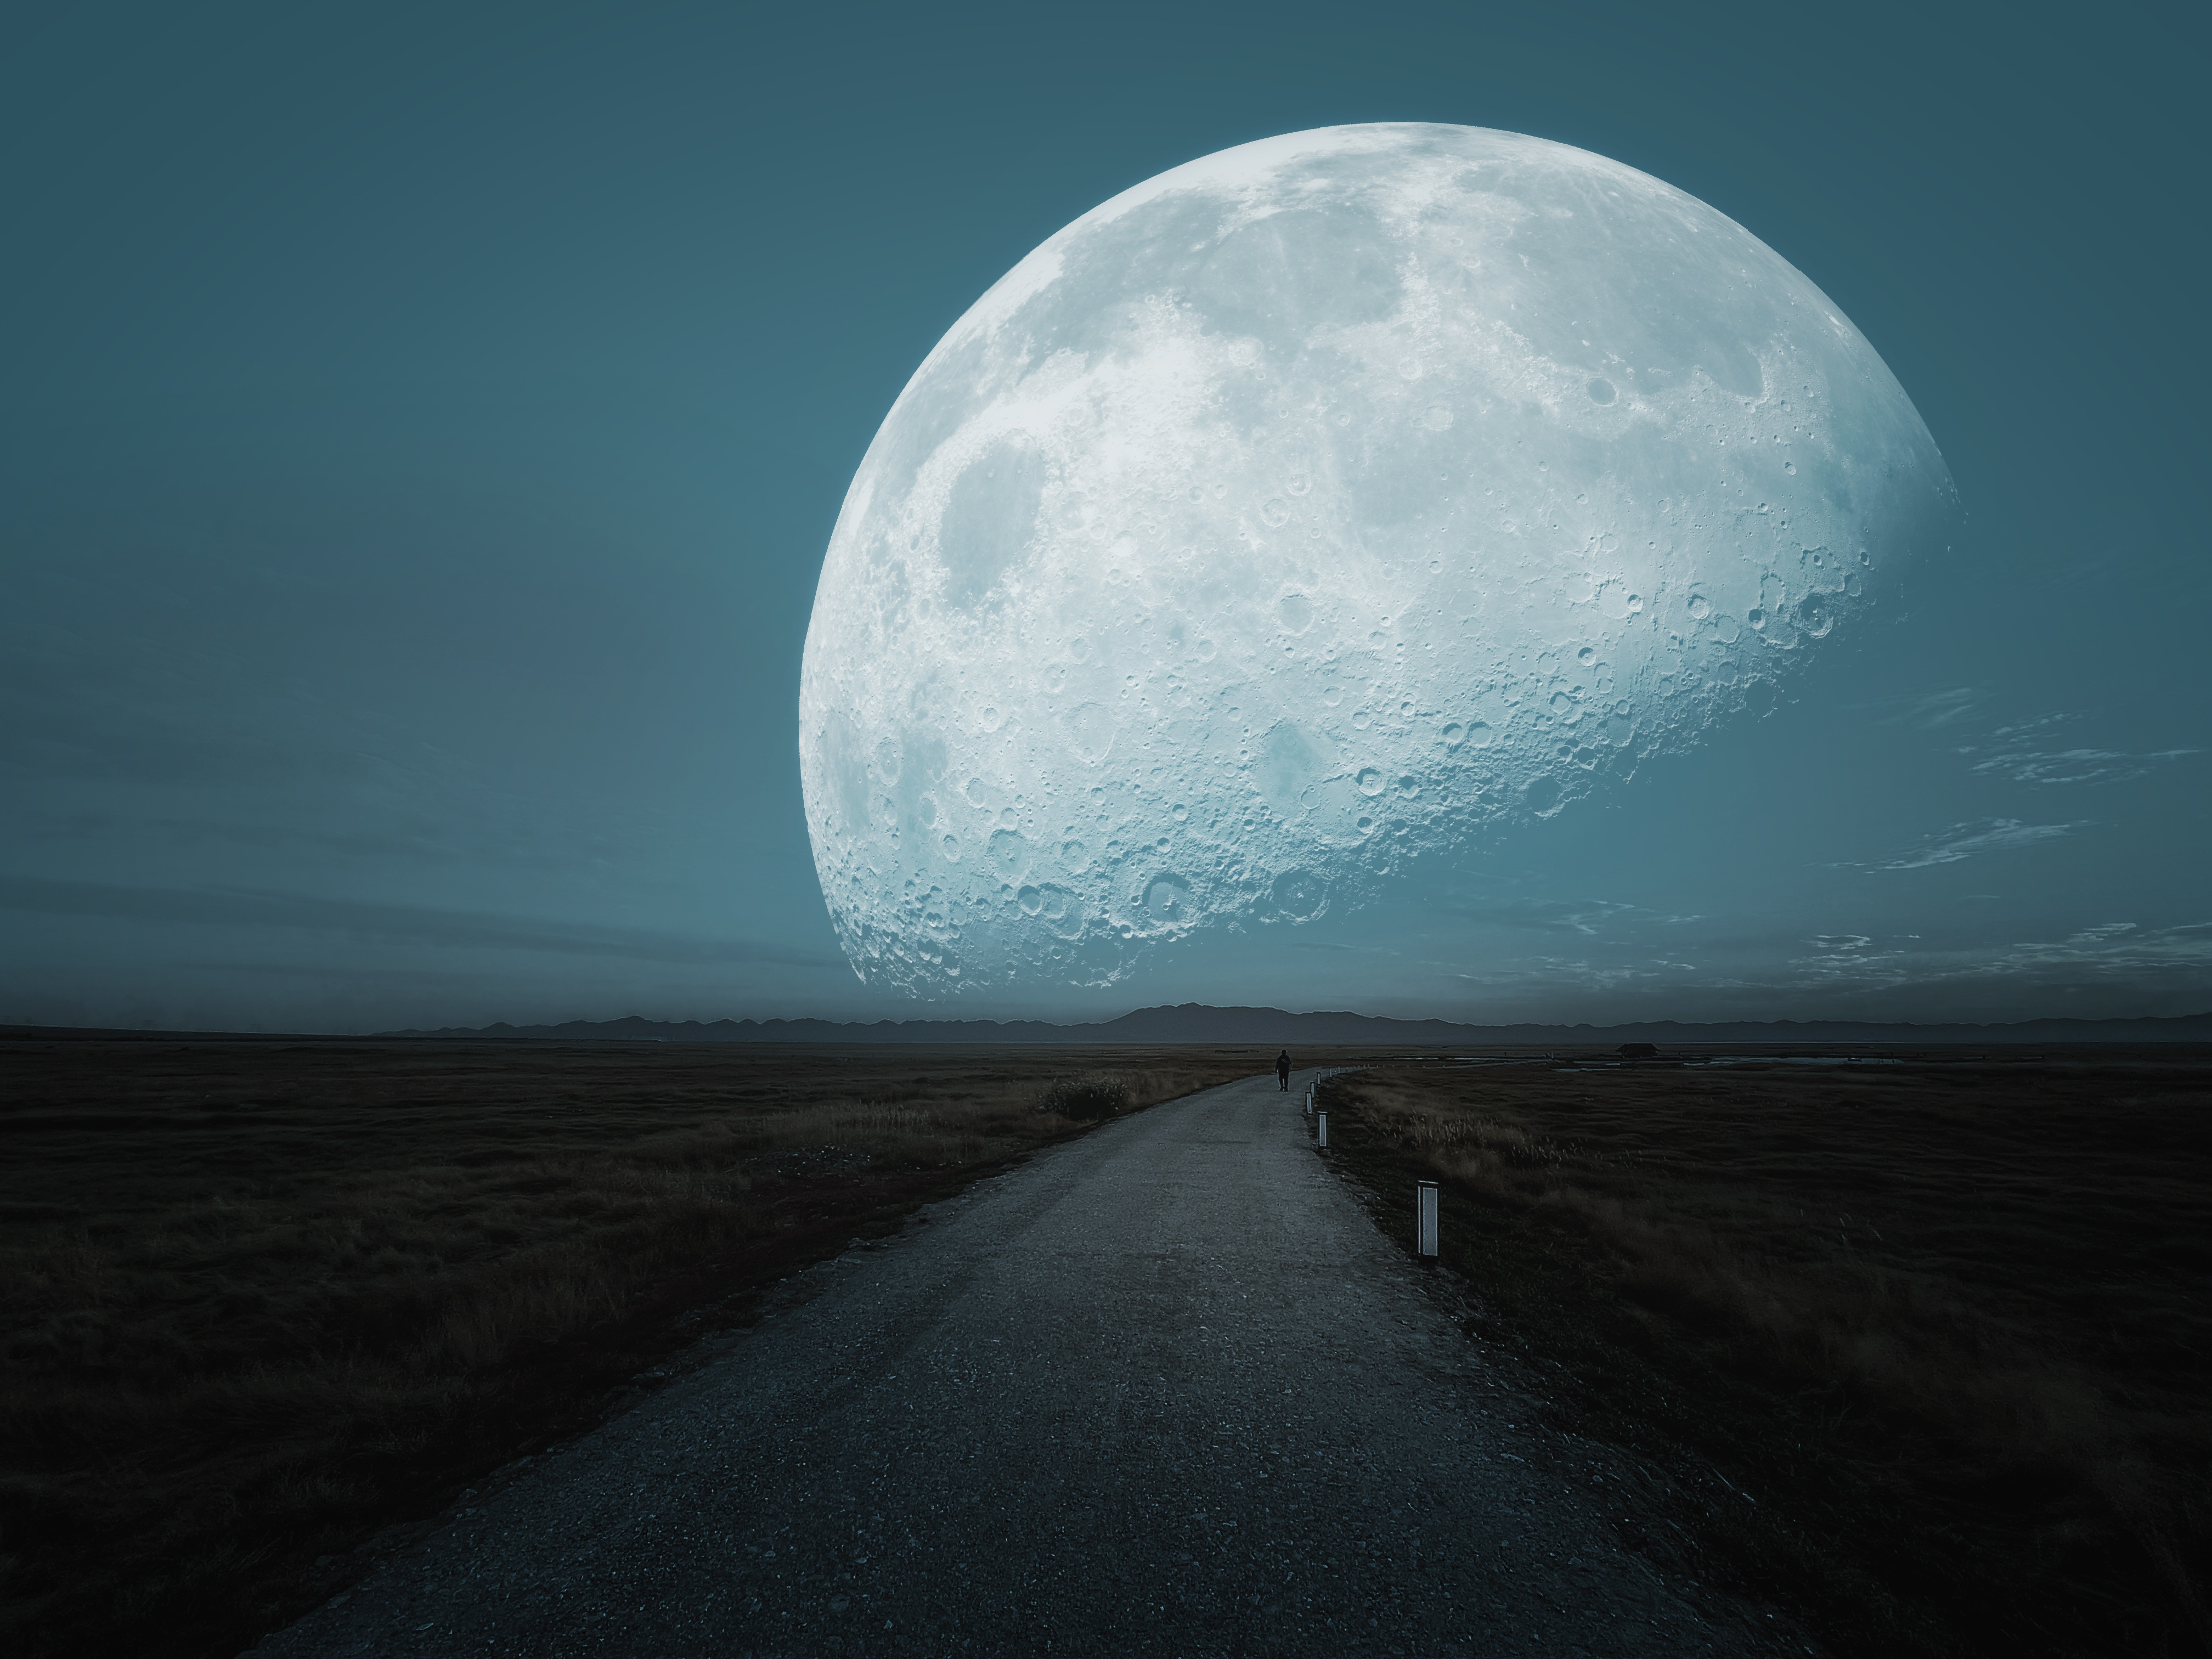
\includegraphics[width=0.8\columnwidth]{figure/comic.jpg}
  \caption*{图 $\_$ 作者}
  \label{fig:comic}
\end{figure}

\newpage
\begingroup % 开启局部组
\thispagestyle{empty} % 仅当前页清空页眉页脚
\restoregeometry
\mybackground
\begin{tikzpicture}[remember picture, overlay]
  % 需要手动调节横向位移
  \node[align=center, xshift=5mm, yshift=2.5cm] at (current page.center){%
    \begin{minipage}{\linewidth}
    \centering
    \fontsize{24}{30}\selectfont\bfseries
    或许你对《GPA》的笑话念念不忘
    \\ 
    又或许你觉得一张纸实在太少
    \\
    所以我们再次为你献上

    \vspace*{2cm}
    {\fontsize{60}{75}\selectfont\bfseries 科幻奇幻笑话}
    \vspace*{2cm}
    
    希望这次够用了
  \end{minipage}
  };
\end{tikzpicture}
\endgroup              % 恢复组外的页眉页脚设置


\newpage
\myheadertext{科幻奇幻笑话}{English Chapter Name |漫画·笑话}
\addcontentsline{toc}{section}{科幻奇幻笑话}

\begin{multicols}{2}
\mybackground
\setlength{\parindent}{0pt}
\subsection*{奇思妙想}
\subsubsection*{1}
社员甲:这是社员尖锐的评论。\\
社员乙:这是社员惊人的嘲讽。\\
社员丙:这是社员装傻的提问。\\
社员丁:这是社员日常的发疯。\\
社员戊:这是社员天才的想法。\\
社员己:这是社员有趣的灵魂。
\subsubsection*{2}
社员甲:这是社员尖锐的评论。\\
社员乙:这是社员惊人的嘲讽。\\
社员丙:这是社员装傻的提问。\\
社员丁:这是社员日常的发疯。\\
社员戊:这是社员天才的想法。\\
社员己:这是社员有趣的灵魂。
\subsubsection*{3}
社员甲:这是社员尖锐的评论。\\
社员乙:这是社员惊人的嘲讽。\\
社员丙:这是社员装傻的提问。\\
社员丁:这是社员日常的发疯。\\
社员戊:这是社员天才的想法。\\
社员己:这是社员有趣的灵魂。

\subsection*{我爱科幻}
\subsubsection*{1}
社员甲:这是社员尖锐的评论。\\
社员乙:这是社员惊人的嘲讽。\\
社员丙:这是社员装傻的提问。\\
社员丁:这是社员日常的发疯。\\
社员戊:这是社员天才的想法。\\
社员己:这是社员有趣的灵魂。
\subsubsection*{2}
社员甲:这是社员尖锐的评论。\\
社员乙:这是社员惊人的嘲讽。\\
社员丙:这是社员装傻的提问。\\
社员丁:这是社员日常的发疯。\\
社员戊:这是社员天才的想法。\\
社员己:这是社员有趣的灵魂。

\subsubsection*{3}
社员甲:这是社员尖锐的评论。\\
社员乙:这是社员惊人的嘲讽。\\
社员丙:这是社员装傻的提问。\\
社员丁:这是社员日常的发疯。\\
社员戊:这是社员天才的想法。\\
社员己:这是社员有趣的灵魂。

\subsection*{三星社团}
\subsubsection*{1}
社员甲:这是社员尖锐的评论。\\
社员乙:这是社员惊人的嘲讽。\\
社员丙:这是社员装傻的提问。\\
社员丁:这是社员日常的发疯。\\
社员戊:这是社员天才的想法。\\
社员己:这是社员有趣的灵魂。
\end{multicols}

\newpage
\mybackground
\begin{multicols}{2}
\setlength{\parindent}{0pt}
社员甲:这是社员尖锐的评论。\\
社员乙:这是社员惊人的嘲讽。\\
社员丙:这是社员装傻的提问。\\
社员丁:这是社员日常的发疯。\\
社员戊:这是社员天才的想法。\\
社员己:这是社员有趣的灵魂。 
\subsubsection*{3}
社员甲:这是社员尖锐的评论。\\
社员乙:这是社员惊人的嘲讽。\\
社员丙:这是社员装傻的提问。\\
社员丁:这是社员日常的发疯。\\
社员戊:这是社员天才的想法。\\
社员己:这是社员有趣的灵魂。
\subsection*{我爱我协}
\subsubsection*{1}
社员甲:这是社员尖锐的评论。\\
社员乙:这是社员惊人的嘲讽。\\
社员丙:这是社员装傻的提问。\\
社员丁:这是社员日常的发疯。\\
社员戊:这是社员天才的想法。\\
社员己:这是社员有趣的灵魂。
\subsubsection*{2}
社员甲:这是社员尖锐的评论。\\
社员乙:这是社员惊人的嘲讽。\\
社员丙:这是社员装傻的提问。\\
社员丁:这是社员日常的发疯。\\
社员戊:这是社员天才的想法。\\
社员己:这是社员有趣的灵魂。
\subsubsection*{3}
社员甲:这是社员尖锐的评论。\\
社员乙:这是社员惊人的嘲讽。\\
社员丙:这是社员装傻的提问。\\
社员丁:这是社员日常的发疯。\\
社员戊:这是社员天才的想法。\\
社员己:这是社员有趣的灵魂。


\end{multicols}

\newpage
\mybackground
\thispagestyle{empty}  % 仅当前页清空页眉页脚
\begin{tikzpicture}[remember picture, overlay]
  \node[align=center, xshift=-5mm] at (current page.center){%
    \begin{minipage}{\linewidth}
    \vspace*{\fill}
\begin{center}
  \scalebox{8.0}{%
    \textcolor{black!30}{%
      \rotatebox{}{\faIcon{poo}}%  
    }%
}
\end{center}
\vfill
  \end{minipage}
  };
\end{tikzpicture}


\newpage
\chapterstartpage{English Chapter Name}{时\\光\\掠\\影}{时光掠影}
\newpage
\myheadertext{交大幻协2002活动记录}{English Chapter Name |交大幻协2002活动记录}
\addcontentsline{toc}{section}{交大幻协2002活动记录}
\setlength{\parindent}{0pt}
\setlength{\parskip}{0pt}
\setlength{\partopsep}{0pt}
\begin{multicols*}{2}

\subsection*{2002.5.22 活动名称}
活动简介

{\bfseries 社员甲:}这是社员尖锐的评论。

{\bfseries 社员乙:}这是社员惊人的嘲讽。

{\bfseries 社员丙:}这是社员装傻的提问。

\begin{center} 
    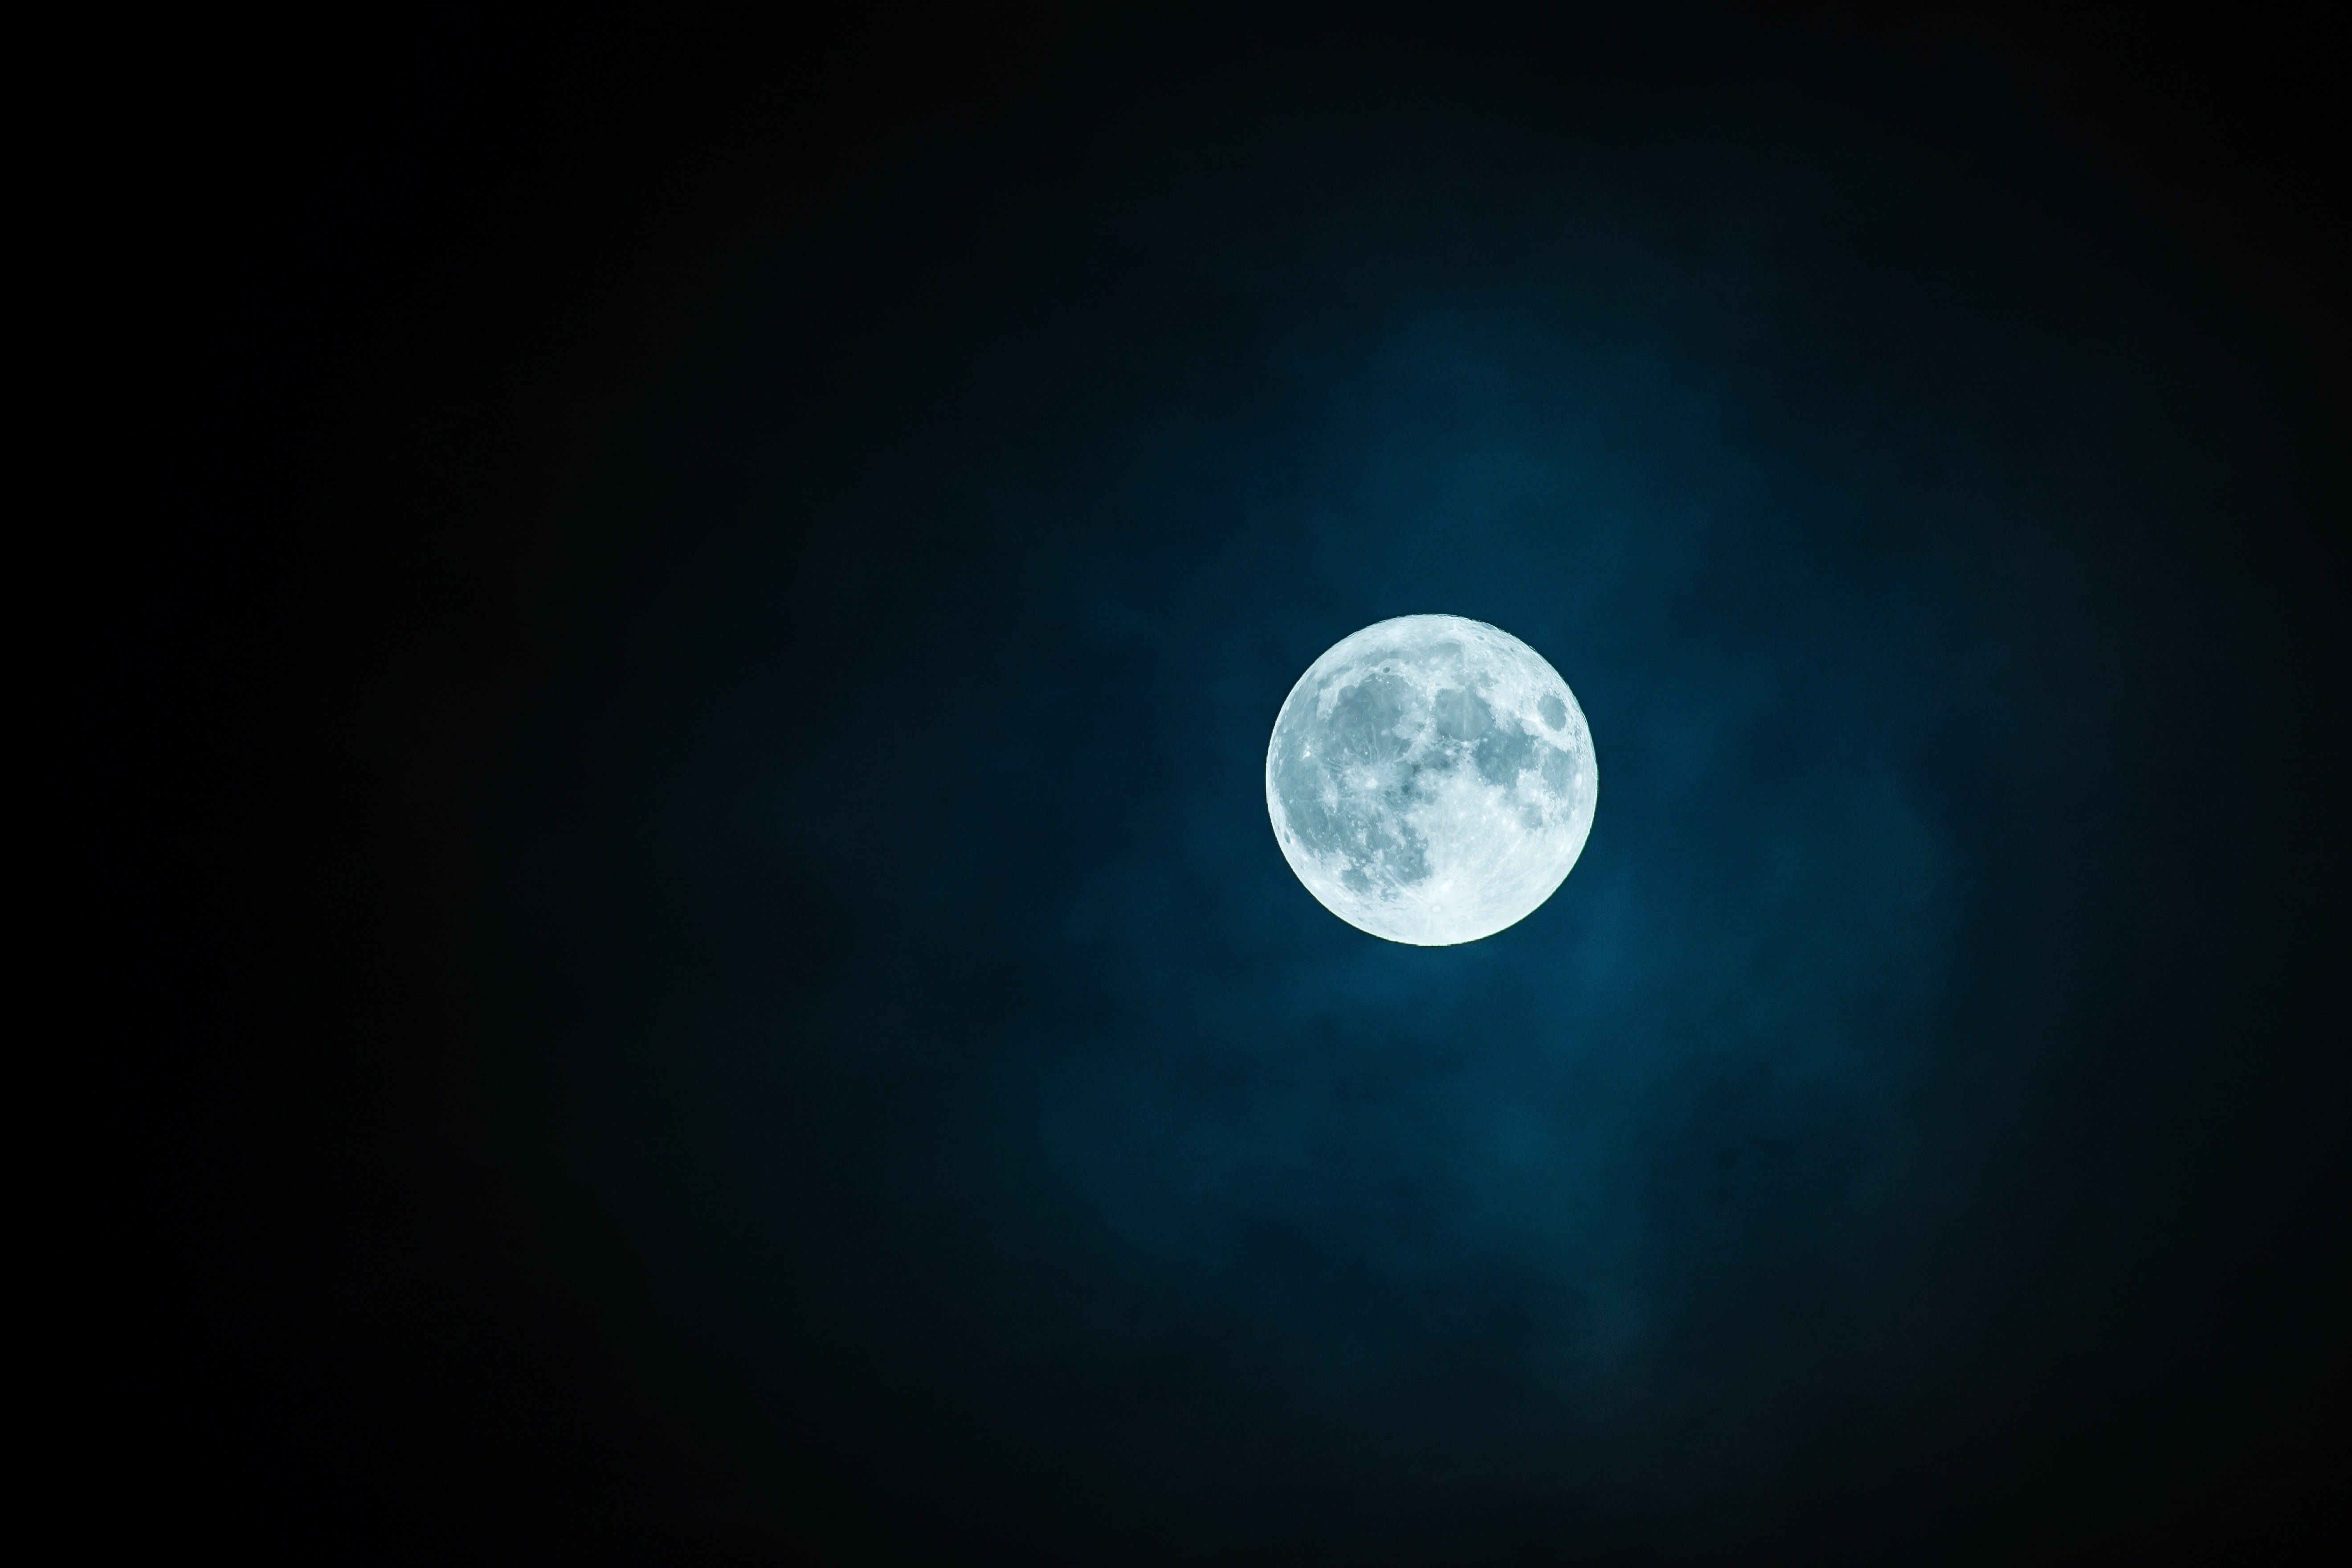
\includegraphics[width=\columnwidth]{figure/images/short.jpg}
    \label{fig:1}
\end{center}
\vspace{-1.25\baselineskip}

{\bfseries 社员甲:}这是社员尖锐的评论。

{\bfseries 社员乙:}这是社员惊人的嘲讽。

{\bfseries 社员丙:}这是社员装傻的提问。

{\bfseries 社员丁:}这是社员日常的发疯。

{\bfseries 社员戊:}这是社员天才的想法。

{\bfseries 社员己:}这是社员有趣的灵魂。


\begin{center}
    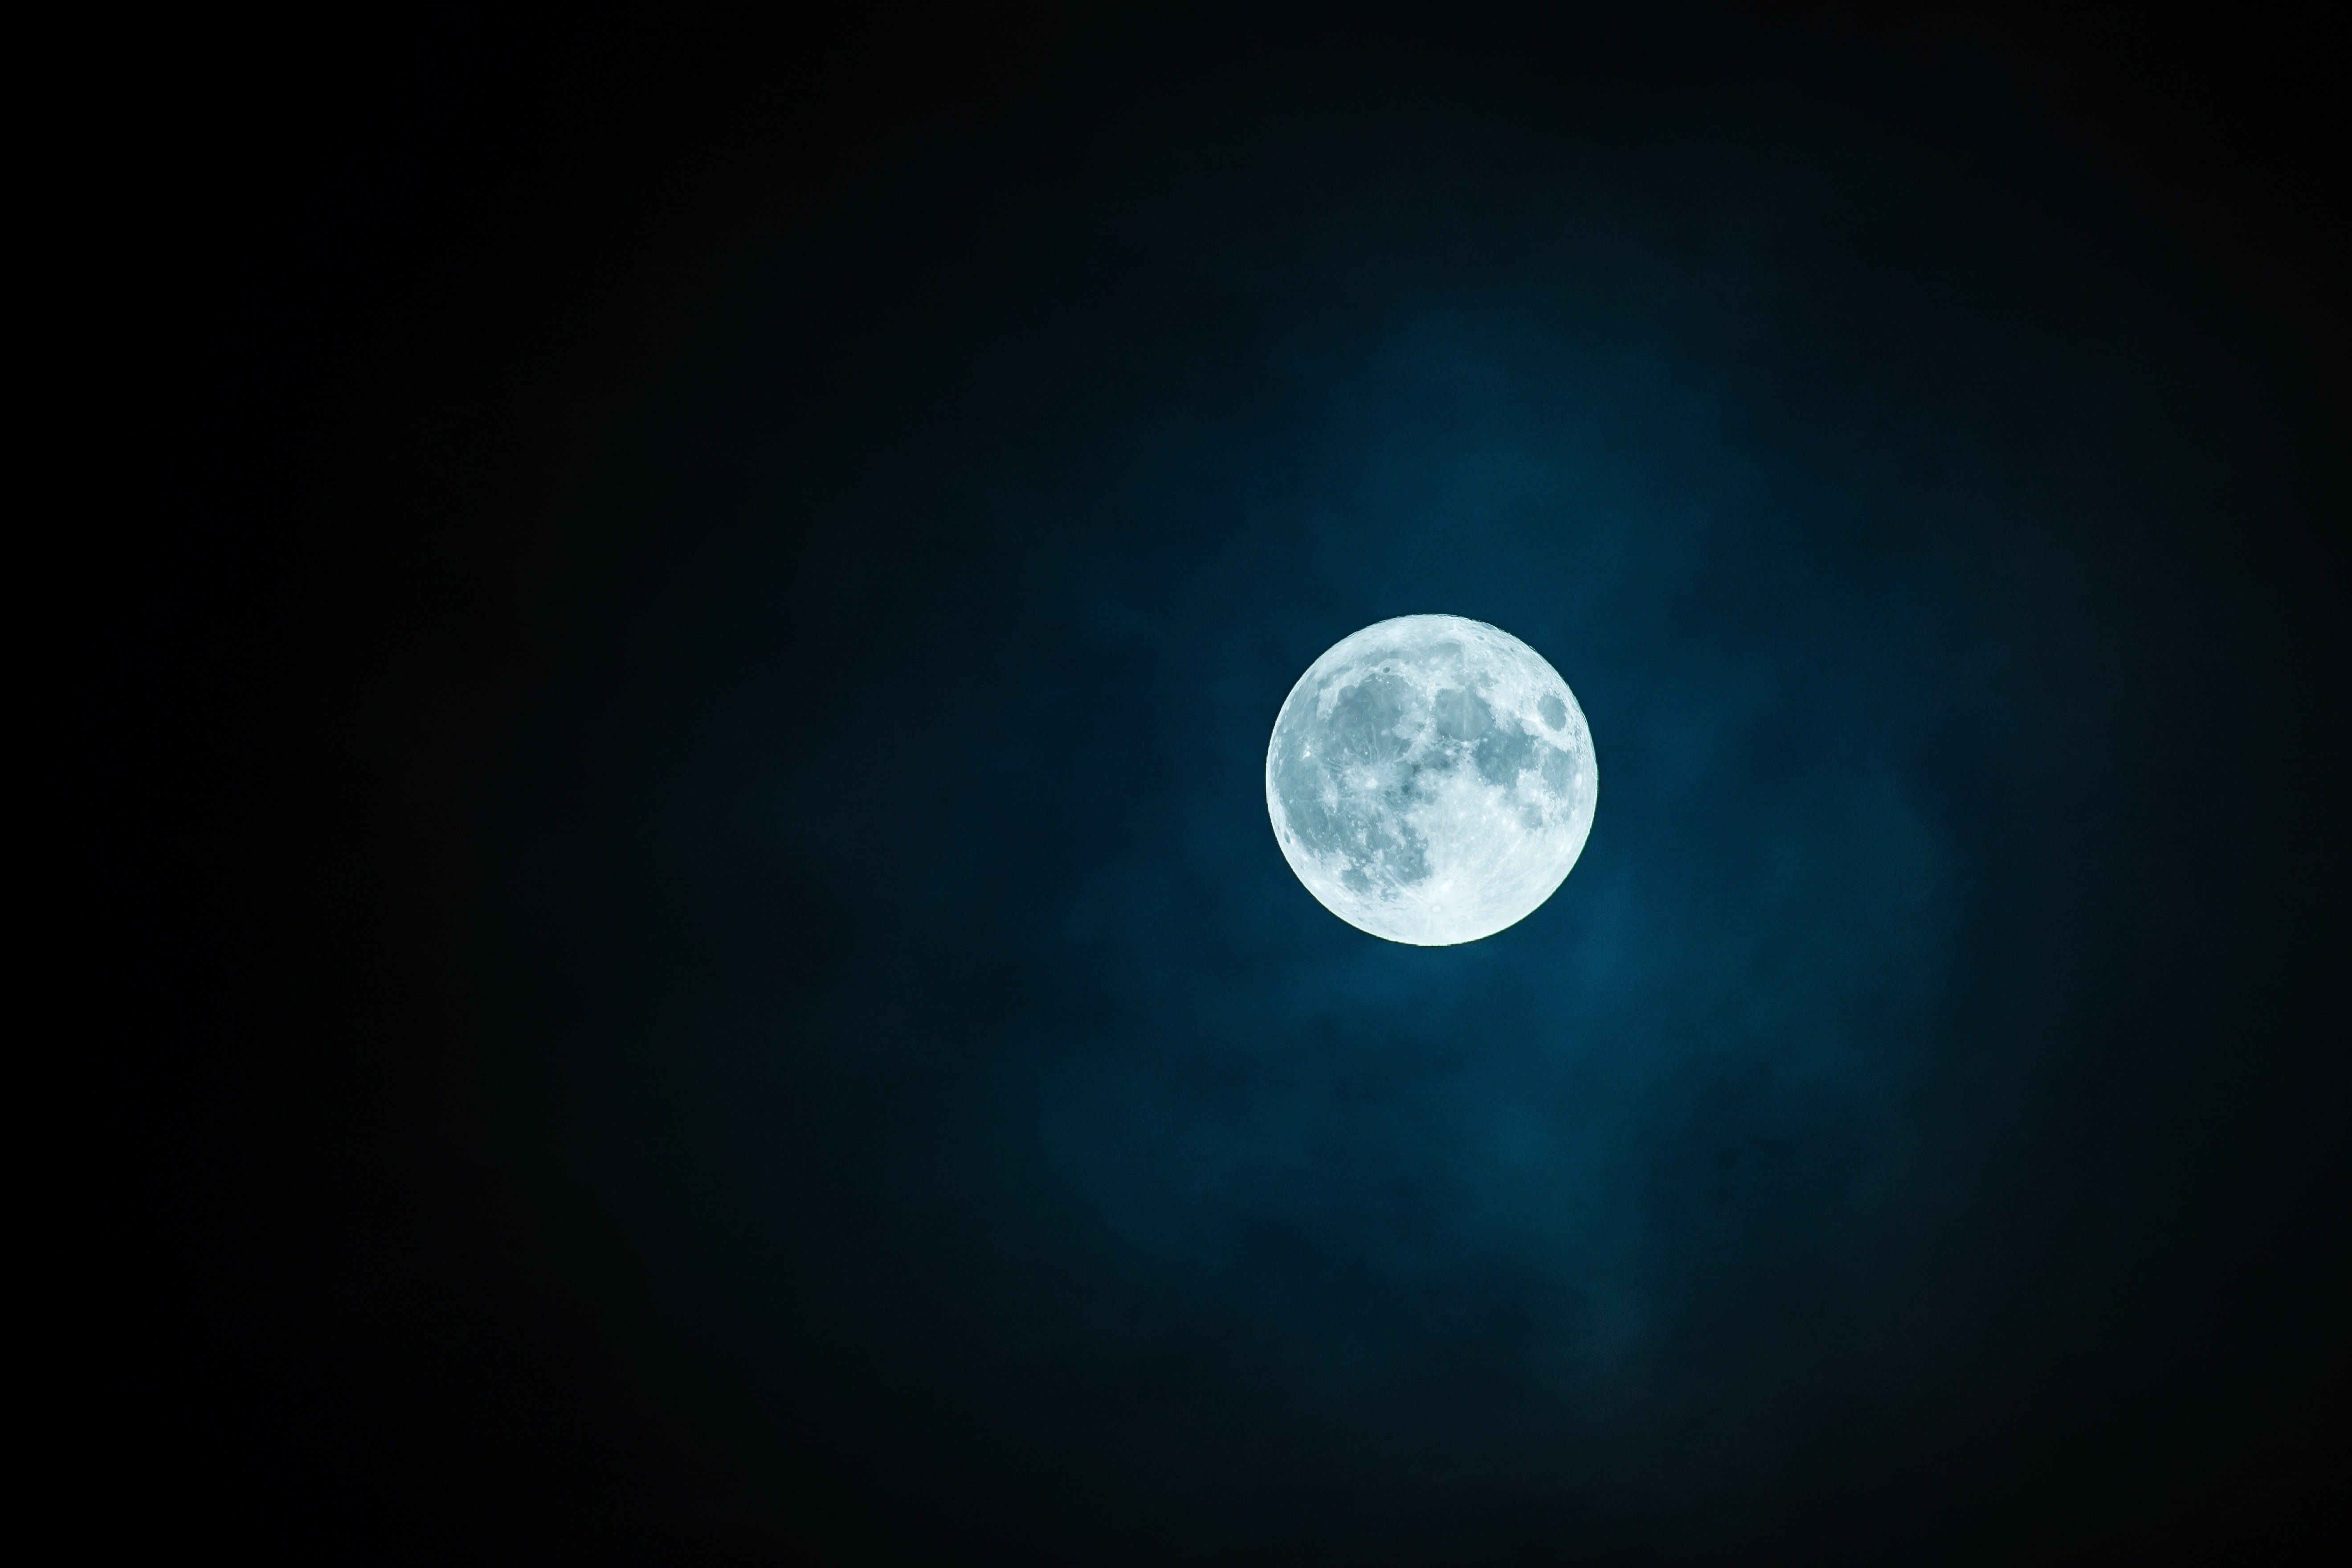
\includegraphics[width=\columnwidth]{figure/images/short.jpg}
    \label{fig:2}
\end{center}

\raggedcolumns

\columnbreak
这是对于无版权图片的描述
\begin{center} 
    \includegraphics[width=\columnwidth]{figure/images/long.jpg}
    \label{fig:3}
\end{center}

\vspace{-1.25\baselineskip}


{\bfseries 社员甲:}这是社员尖锐的评论。


\begin{center}
    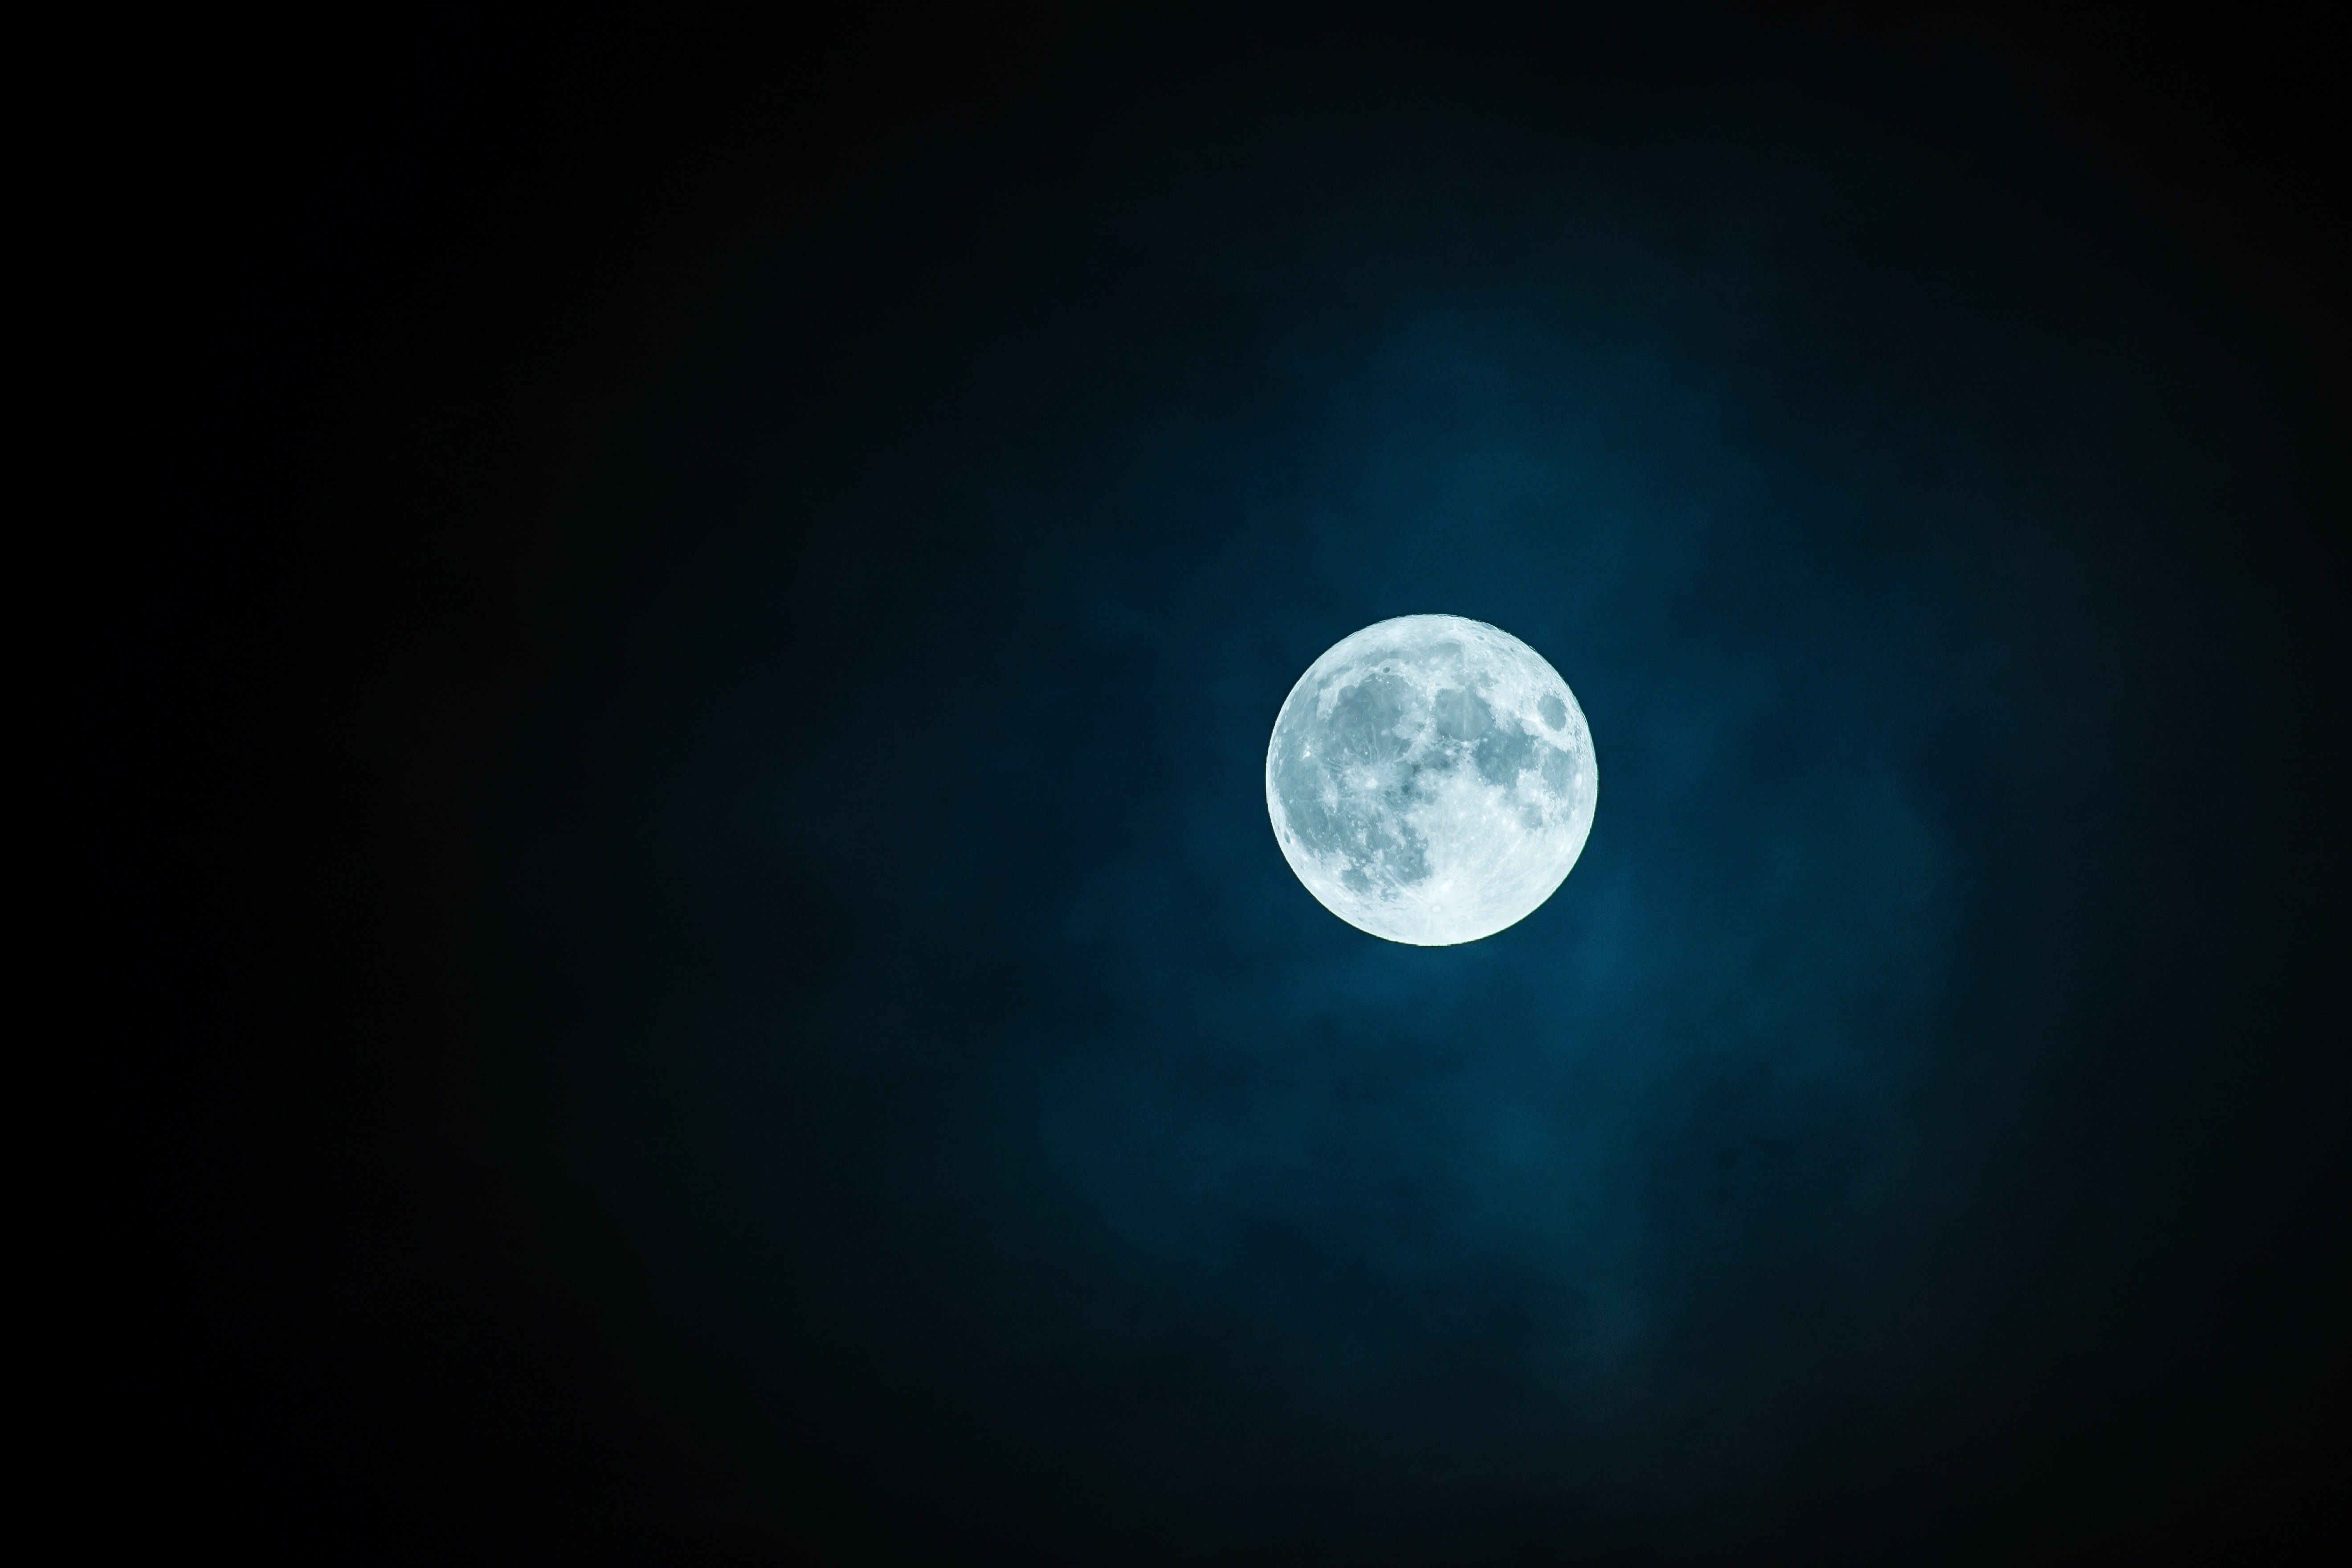
\includegraphics[width=\columnwidth]{figure/images/short.jpg}
    \label{fig:20240928-4}
\end{center}

\end{multicols*}

%%--------------------空白页--------------------%%
\clearpage
\thispagestyle{empty} % 只影响当前页
\null
\newpage


%%--------------------尾页--------------------%%
\newpage
\thispagestyle{empty}

\vspace*{\fill}

\noindent
\begin{tabularx}{\linewidth}{@{}lX@{}}
  \begin{tabular}[c]{l @{\quad} l}
    创意策划: & 交大幻协第二十一届全体核心成员 \\
    文字编辑: & 名字 \\
    美术编辑: & 名字 \\
    封面设计: & 名字 \\
    封面摄影: & 名字 \\
    社徽设计: & 名字 \\
  \end{tabular}
  &
  \centering
   \raisebox{-12mm}{%
    \scalebox{8}{\faRocket} % 社徽
  }
\end{tabularx}

\vspace{0.5in}



\end{document}